%Olli
\section{Architektur}
In diesem Kapitel wird die Software Architektur des Projektes vorgestellt. Das
Spiel wurde nach dem ``MVC'' (Model View Controller) Konzept entwickelt. Das bedeutet,
dass die Klassen, die das Modell und dessen Daten darstellen, sowohl das View
als auch den Controller nicht kennen. Das View, das in diesem Fall die
graphische Benutzeroberfl�che ist kennt hingegen zwar das Modell, den
Controller aber nicht. Diese Trennung ist wichtig, damit die Datenhaltung und
Logik seperat von der graphischen Benutzeroberfl�che entwickelt werden kann.

Der Controller kennt beide anderen Ebenenen und
verwaltet diese --- es sorgt beispielsweise daf�r, dass die Benutzeroberfl�che
immer die aktuellen Daten anzeigt. In unserem Projekt wird der Controller durch
eine einzelne Klasse gebildet, die das Singleton Pattern implementiert. Dadurch
kann jede Klasse statisch auf den Controller zugreifen, ohne eine Referenz zu
ihm speichern zu m�ssen --- und trotzdem kann der Controller objektorientiert
entwickelt werden. %Das hier eher = Implementierung?

%MVC Bild
\begin{figure}[H]
\centering
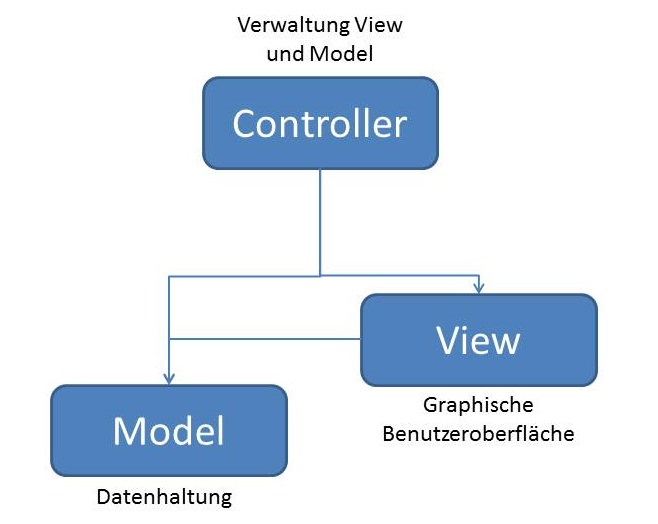
\includegraphics[width=0.5\textwidth]{se-wa-jpg/mvc}
\caption{Model View Controller Konzept}
\label{MVC Konzept}
\end{figure}

Es wurde fr�h entschieden, dass das Spiel nicht nur auf einem Computer
laufen soll (``Hotseat''), sondern dass das Spiel von einem Server kontrolliert
wird und die Daten an Clients, die auf unterschiedlichen Computern
laufen k�nnen, verschickt werden --- somit k�nnen die Spieler gleichzeitig
spielen und haben keine langen Wartephasen. Prim�r befindet sich die Logik des
Spiels und die Datenhaltung dabei zentral auf dem Server.

Des Weiteren wurde keine persistente Speicherung der Spieldaten vorgesehen.
Sobald der Server also nicht mehr l�uft sind die Daten des aktuellen Spiels
verloren. Dies reduziert die Komplexit�t des Modells, denn es muss beim
Initialisieren des Spiels keine Daten laden und beim Beenden des Spiels keine
Daten speichern.

